\documentclass{article}
\usepackage{ctex} % 添加中文支持包
\usepackage{geometry}
\geometry{margin=2.5cm}
\usepackage{graphicx}
\usepackage{mhchem}
\usepackage{amsmath}
\usepackage{booktabs}
\usepackage{hyperref}
\usepackage{graphicx}
\usepackage{float}
\usepackage{subcaption}
\usepackage{xcolor}

\title{Ex13}

\begin{document}
\newpage

\section{状态变量、输入变量，输出变量}

状态变量7个\newline\newline
    1   {       'Uc\_Cp'                    }\newline
    2   {       'Uc\_Cps'                   }\newline
    3   {       'Uc\_Cs'                    }\newline
    4   {       'Il\_Lph1'                  }\newline
    5   {       'Il\_Lph2'                  }\newline
    6   {       'Il\_Ls'                    }\newline
    7   {       'Il\_Lm：Linear Transformer'              }\newline
    

\indent 输入变量18个\newline\newline
    1   {      'I\_S1/Ideal Switch'         }\newline
    2   {      'I\_S2/Ideal Switch'         }\newline
    3   {      'I\_S3/Ideal Switch'                }\newline
    4   {      'I\_S4/Ideal Switch'                }\newline
    5   {      'I\_S5/Ideal Switch'                }\newline
    6   {      'I\_S6/Ideal Switch'                }\newline
    7   {      'I\_S7/Ideal Switch'                }\newline
    8   {      'I\_S8/Ideal Switch'                }\newline
    9   {      'I\_S1/Diode'         }\newline
    10   {      'I\_S2/Diode'         }\newline
    11   {      'I\_S3/Diode'                }\newline
    12   {      'I\_S4/Diode'                }\newline
    13   {      'I\_S5/Diode'                }\newline
    14   {      'I\_S6/Diode'                }\newline
    15   {      'I\_S7/Diode'                }\newline
    16   {      'I\_S8/Diode'                }\newline
    17   {      'U\_Udc1'    }\newline
    18   {      'U\_Udc2'        }\newline

\indent 输出变量18个\newline\newline
    1   {      'U\_S1/Ideal Switch'         }\newline
    2   {      'U\_S2/Ideal Switch'         }\newline
    3   {      'U\_S3/Ideal Switch'                }\newline
    4   {      'U\_S4/Ideal Switch'                }\newline
    5   {      'U\_S5/Ideal Switch'                }\newline
    6   {      'U\_S6/Ideal Switch'                }\newline
    7   {      'U\_S7/Ideal Switch'                }\newline
    8   {      'U\_S8/Ideal Switch'                }\newline
    9   {      'U\_S1/Diode'         }\newline
    10   {      'U\_S2/Diode'         }\newline
    11   {      'U\_S3/Diode'                }\newline
    12   {      'U\_S4/Diode'                }\newline
    13   {      'U\_S5/Diode'                }\newline
    14   {      'U\_S6/Diode'                }\newline
    15   {      'U\_S7/Diode'                }\newline
    16   {      'U\_S8/Diode'                }\newline
    17   {      'U\_Voltage Measurement'    }\newline
    18   {      'U\_Voltage Measurement1'        }\newline
    19   {      'I\_Current Measurement'        }\newline

\section{simulink建模}
\begin{figure}[H] % 使用[H]选项将图片固定在当前位置
    \centering
    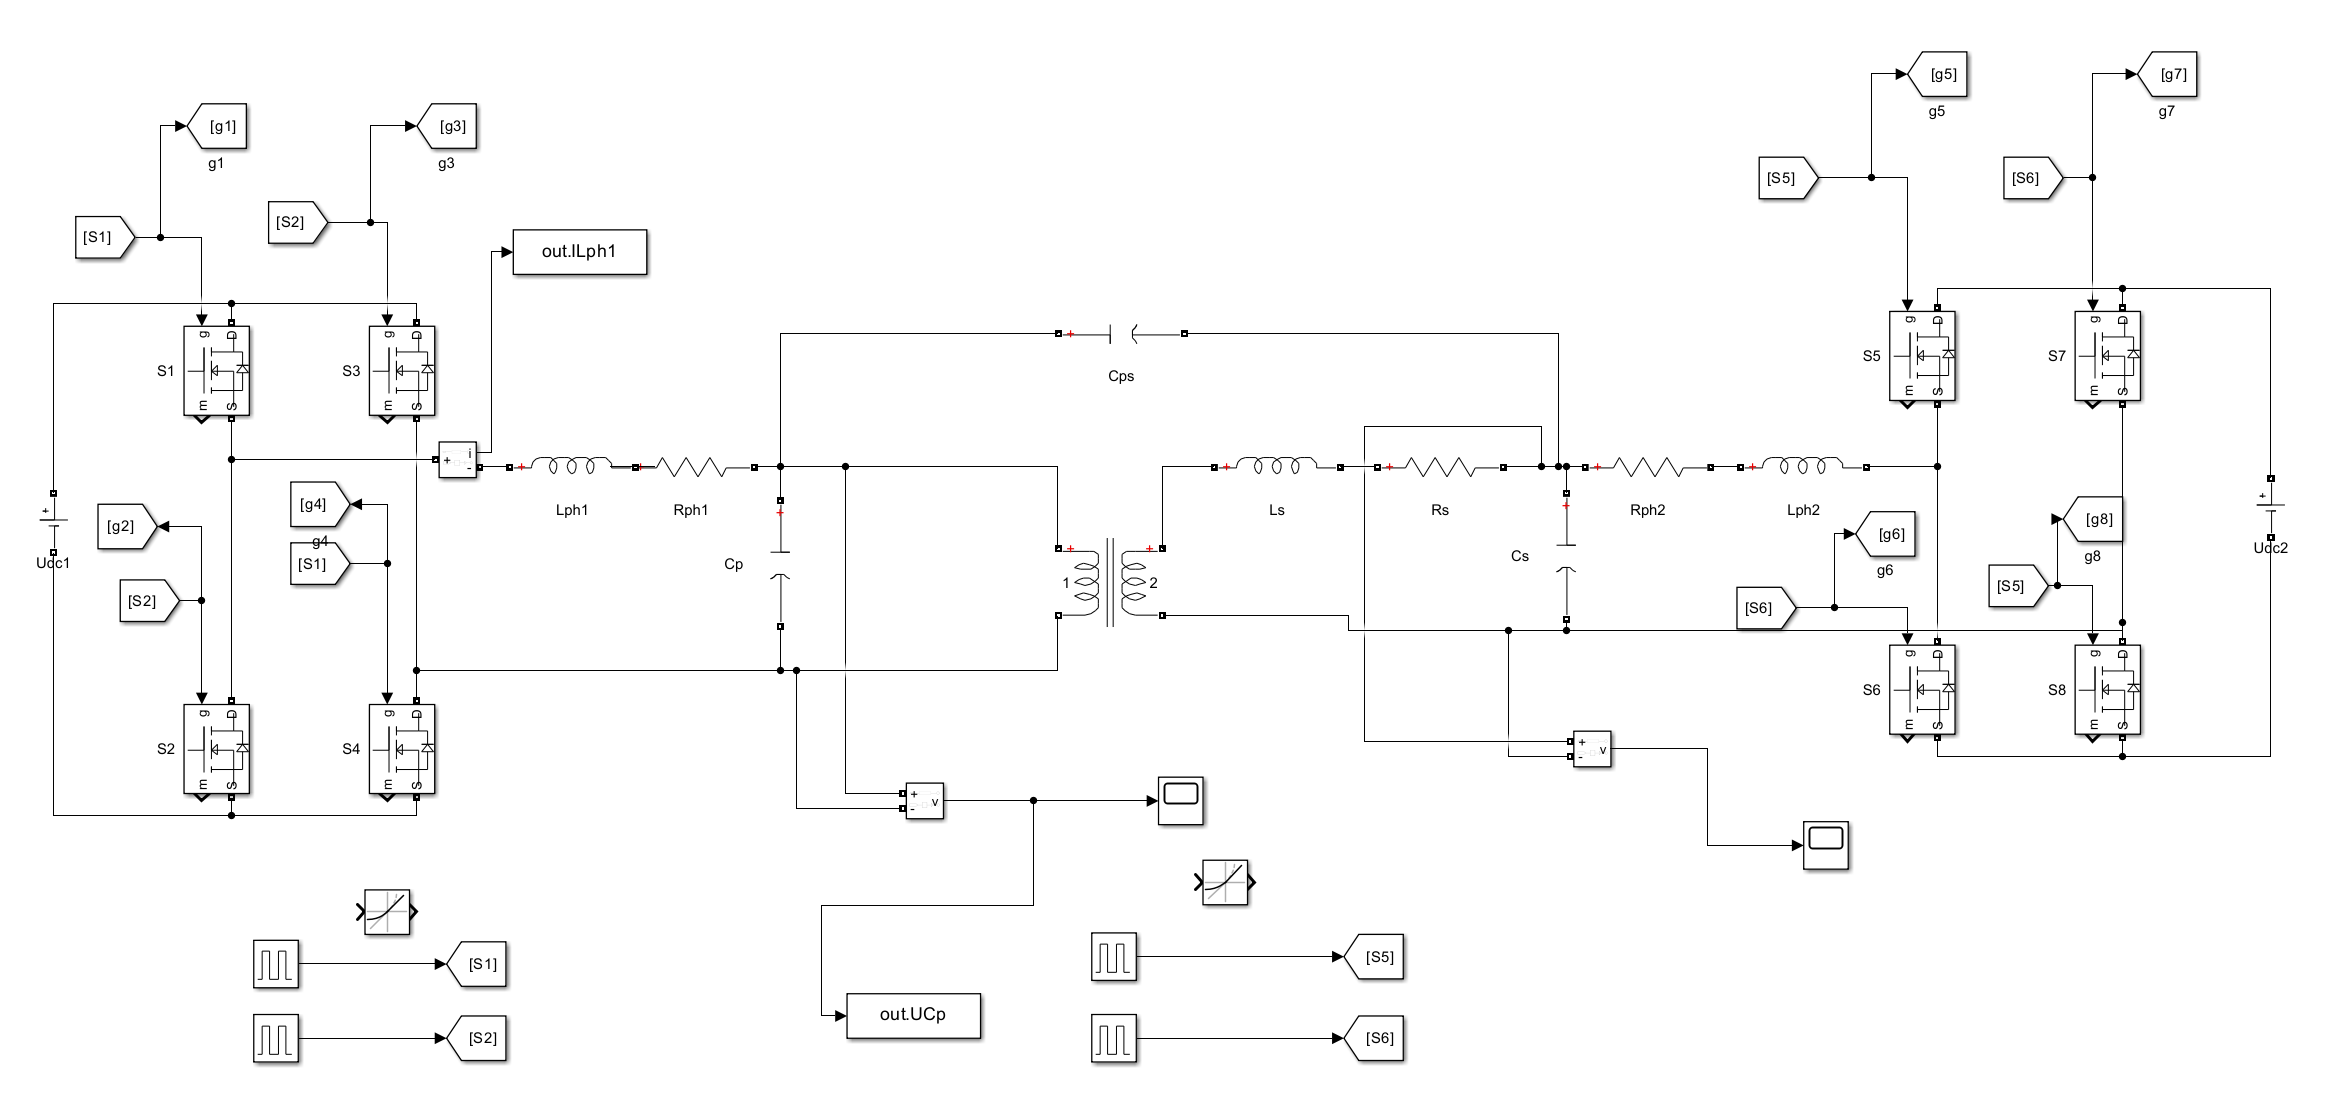
\includegraphics[width=1.0\textwidth]{sim_construct.png}
    \caption{simmulink模型}
    \label{fig:motor_structures}
\end{figure}

\newpage
\section{控制信号}

\indent S1和S4控制信号相同：\newline
\indent g1=g4 (方波，周期100e-6秒，占空比50\%，相位延迟0秒)\newline \newline
\indent S2和S3控制信号相同(与S1、S4互补)：\newline
\indent g2=g3 (方波，周期100e-6秒，占空比50\%，相位延迟50e-6秒)\newline \newline

\indent S5和S8控制信号相同(延迟S1、S4四分之一周期)：\newline
\indent g5=g8 (方波，周期100e-6秒，占空比50\%，相位延迟25e-6秒)\newline \newline
\indent S6和S7控制信号相同(与S5、S8互补)：\newline
\indent g6=g7 (方波，周期100e-6秒，占空比50\%，相位延迟75e-6秒)\newline \newline

\section{转换矩阵Req}
\begin{figure}[H] % 使用[H]选项将图片固定在当前位置
    \centering
    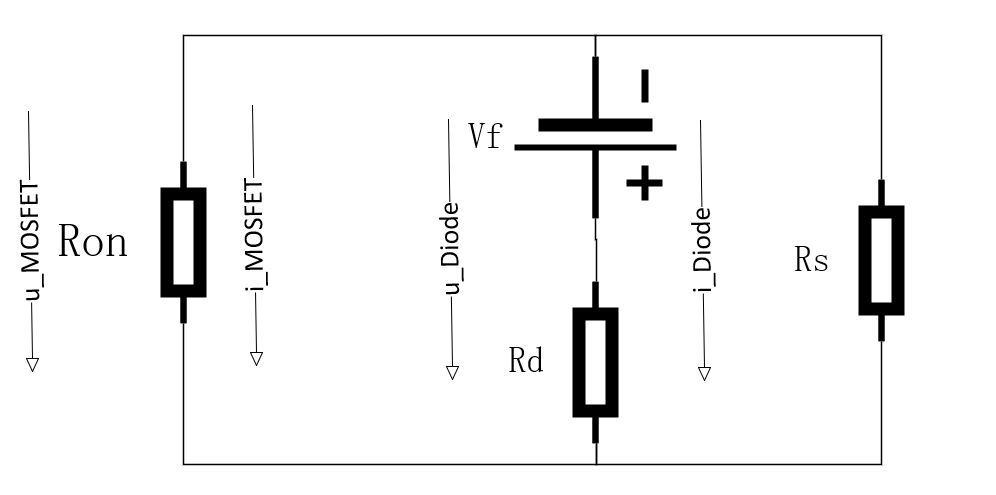
\includegraphics[width=0.8\textwidth,height=0.4\textwidth]{trans.png}
    \caption{MOSFET和Diode示意图}
    \label{fig:motor_structures}
\end{figure}

\indent MOSFET导通时: \indent $u_{MOSFET} = R_{on} \times i_{MOSFET}$\newline
\indent MOSFET截止时：\indent $i_{MOSFET} = 0$\newline
\indent Diode导通时：\indent $u_{Diode} = R_{d} \times i_{Diode} - V_{f}$\newline
\indent Diode截止时：\indent $i_{Diode} = 0$\newline



\newpage
\section{MOSFET和Diode导通状态判断}
\indent (g1,g2,g3,g4)控制信号仅有三种情况(1,0,0,1)、(0,1,1,0)、(0,0,0,0)\newline
\indent (g5,g6,g7,g8)控制信号与(g1,g2,g3,g4)处理方法相同。

\begin{figure}[H] % 使用[H]选项将图片固定在当前位置
    \centering
    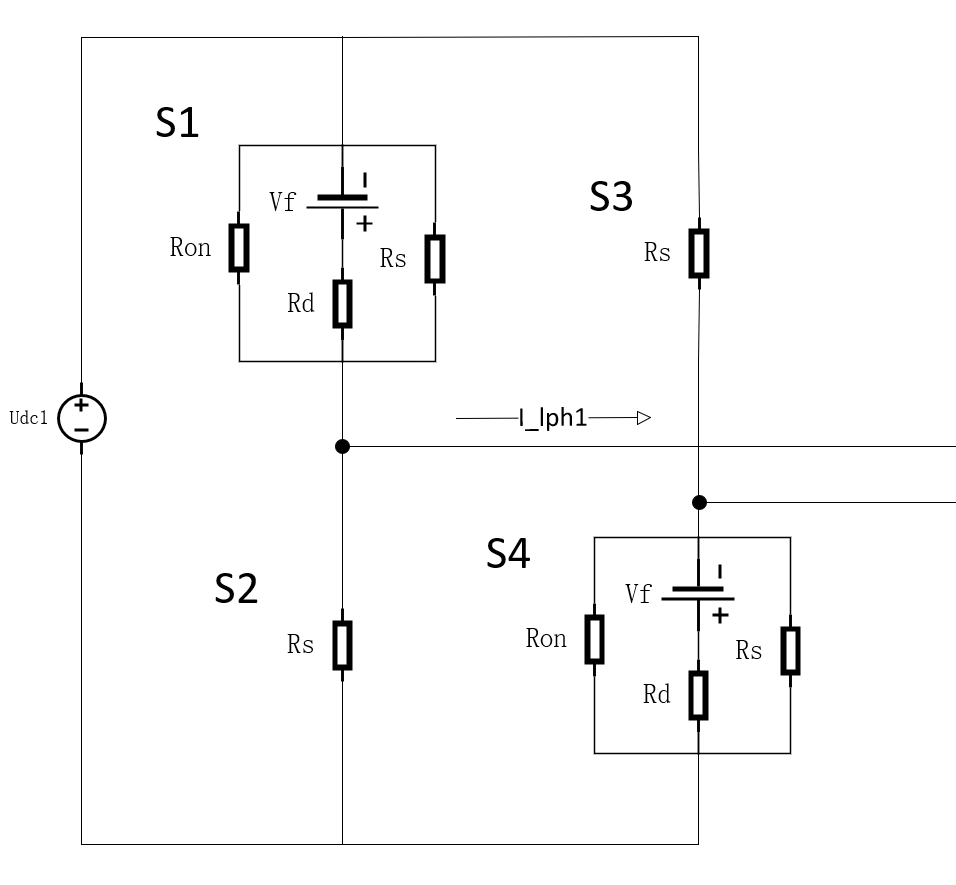
\includegraphics[width=0.8\textwidth]{state.png}
    \caption{控制信号(g1,g2,g3,g4)=(1,0,0,1)情况}
    \label{fig:motor_structures}
\end{figure}

\indent S1-MOSFET 导通\newline
\indent S2-MOSFET 截止\newline
\indent S3-MOSFET 截止\newline
\indent S4-MOSFET 导通\newline
\indent S1-Diode 若I\_lph1流出($>0$)则截止，若I\_lph1流入($<0$)则导通(Vf=0)\newline
\indent S2-Diode 截止\newline
\indent S3-Diode 截止\newline
\indent S4-Diode 若I\_lph1流出($>0$)则截止，若I\_lph1流入($<0$)则导通(Vf=0)\newline\newline

\indent (g1,g2,g3,g4)=(0,0,0,0) 情况仅在开始时可能存在，桥所有MOSFET和Diode均截止。

\newpage
\section{仿真结果}

\begin{figure}[H] % 使用[H]选项将图片固定在当前位置
 \centering
    \begin{minipage}{1.0\textwidth}
        \centering
         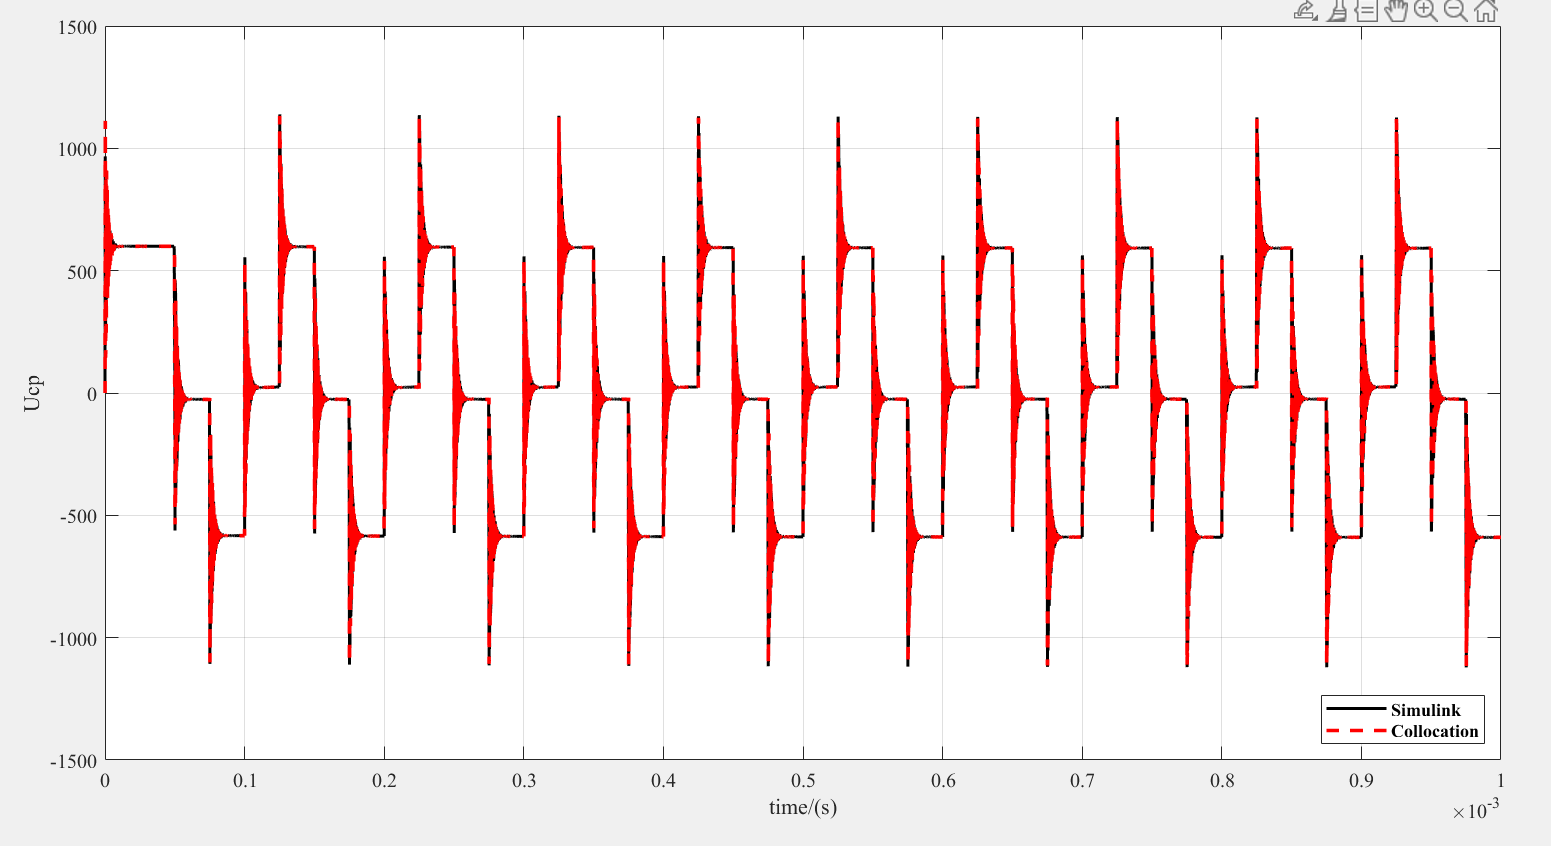
\includegraphics[width=\textwidth, height=0.5\textwidth, keepaspectratio]{Ucp.png}
        
        \label{fig:rotor}
    \end{minipage}
    \hfill
    \begin{minipage}{1.0\textwidth}
        \centering
        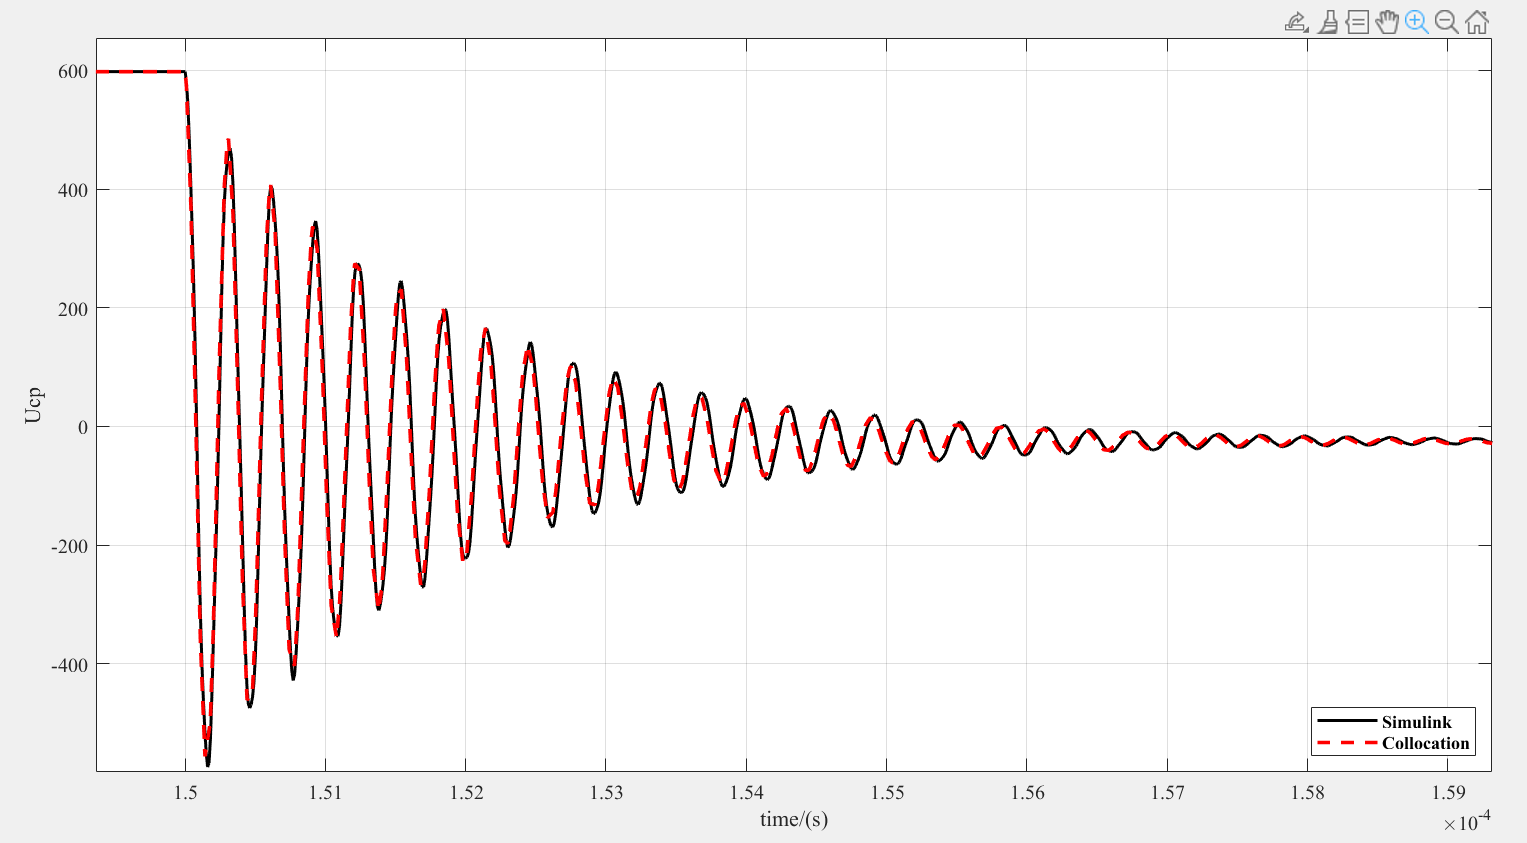
\includegraphics[width=\textwidth, height=0.5\textwidth, keepaspectratio]{Ucp_detail.png}
        
        \label{fig:stator}
    \end{minipage}
    
    \caption{Ucp-时间图像}
    \label{fig:motor_structures}
\end{figure}

\begin{figure}[H] % 使用[H]选项将图片固定在当前位置
 \centering
    \begin{minipage}{1.0\textwidth}
        \centering
         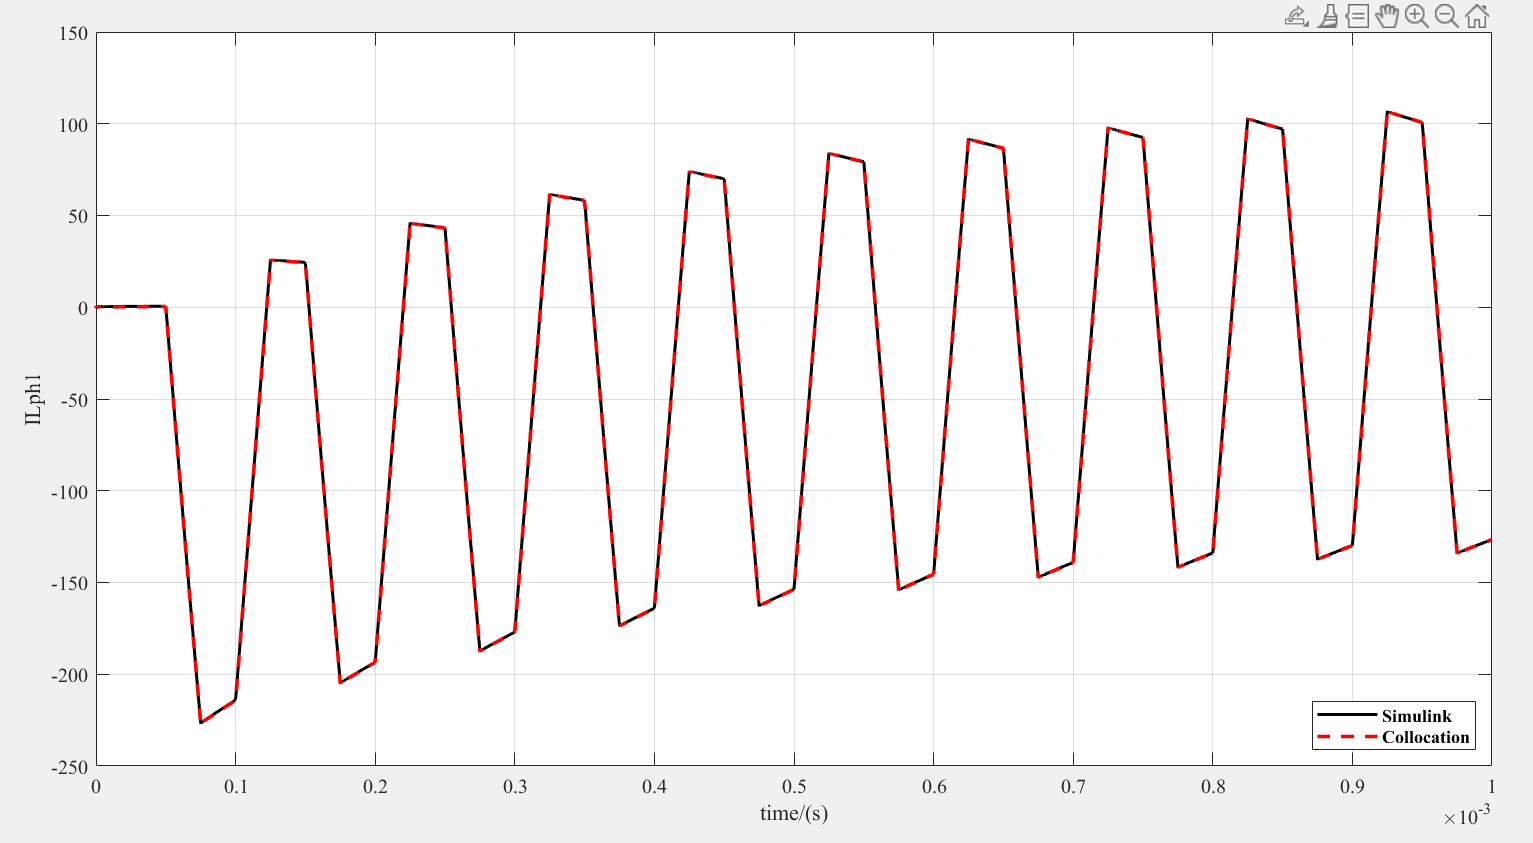
\includegraphics[width=\textwidth, height=0.5\textwidth, keepaspectratio]{ILph1.png}
        
        \label{fig:rotor}
    \end{minipage}
    \hfill
    \begin{minipage}{1.0\textwidth}
        \centering
        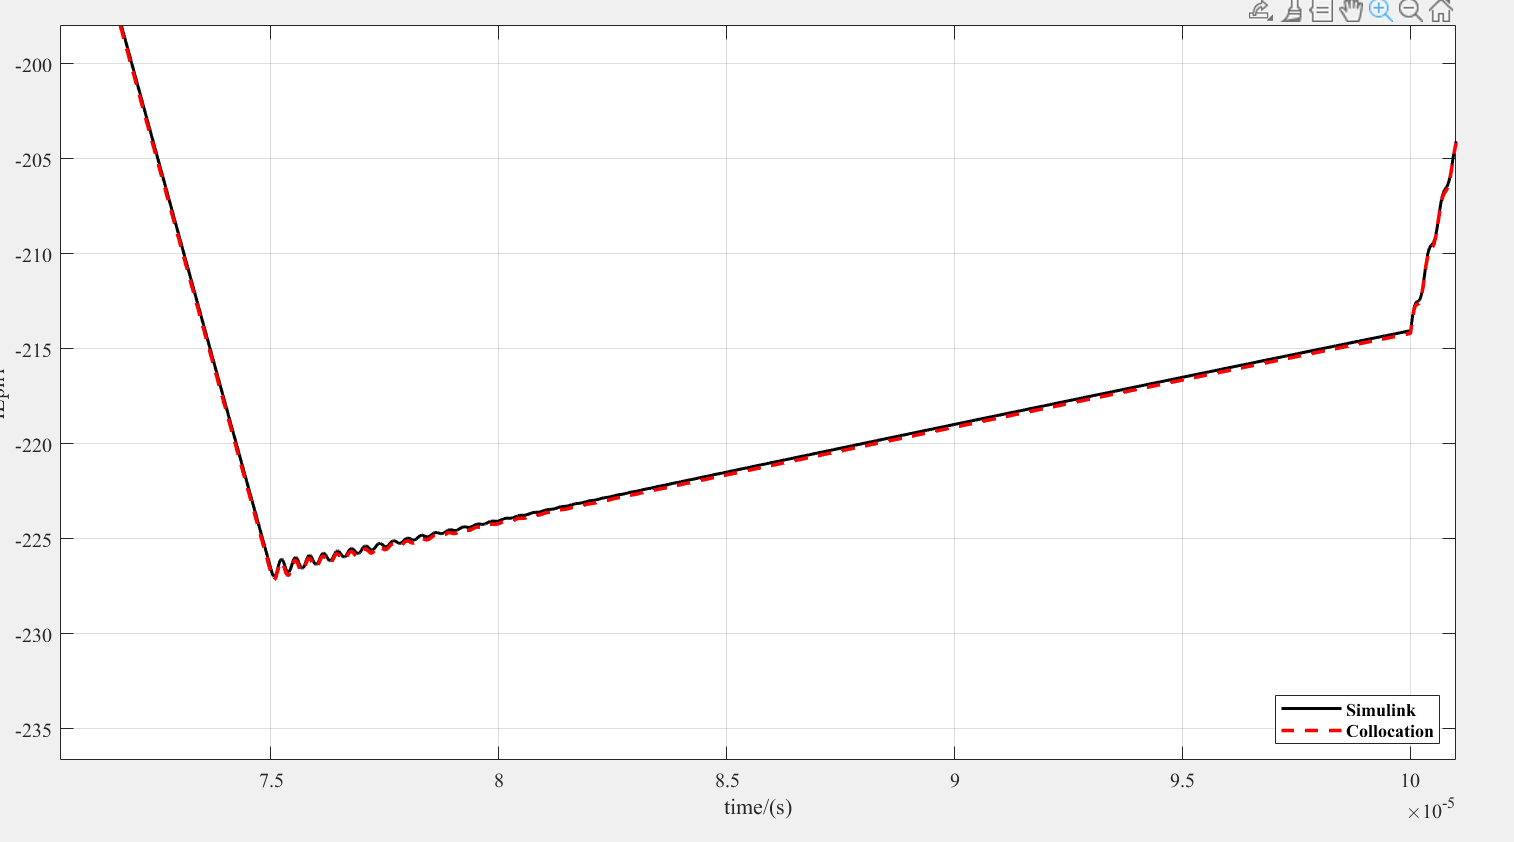
\includegraphics[width=\textwidth, height=0.5\textwidth, keepaspectratio]{ILph1_detail.png}
        
        \label{fig:stator}
    \end{minipage}
    
    \caption{ILph1-时间图像}
    \label{fig:motor_structures}
\end{figure}

\end{document}
